\documentclass{beamer}
\graphicspath{{../graphics/}}
\usepackage{listings}
\usepackage{ulem}
\usepackage{subcaption}
\captionsetup{compatibility=false}
\usepackage[linesnumbered]{algorithm2e}
\usepackage{multicol}

\newcommand{\linespace}{\vspace{1em}}

\mode<presentation>
{
  \usetheme{Darmstadt}
  \setbeamertemplate{footline}[frame number]
  \setbeamertemplate{navigation symbols}{}
  \setbeamercovered{transparent}
}

\AtBeginSection[]
{
   \begin{frame}
        \frametitle{Indhold}
        \tableofcontents[sectionstyle=show/hide,subsectionstyle=show/show/hide]
   \end{frame}
}

\usepackage[danish]{babel}
\usepackage[T1]{fontenc}

\usepackage[utf8]{inputenc}

\usepackage{times}

\usepackage{tikz}
\usepackage{multirow}

\title[Stemmespillet]{Stemmespillet (Cars)}

\subtitle{SW613F14}

\author[SW613F14]{
Mikael Elkiær Christensen \\\and
Mikkel Sandø Larsen \\\and
Stefan Marstrand Getreuer Micheelsen \\\and
Bruno Thalmann
}

\institute[Aalborg Universitet]
{
  Software\\
  Aalborg Universitet}

\date[CFP 2003]{16. juni 2014}

\begin{document}

%--------------------------------------------------
%     INTRODUKTION
%--------------------------------------------------

\begin{frame}
  \titlepage
\end{frame}

\begin{frame}
    \frametitle{Indhold}
    \tableofcontents[sectionstyle=show/show,subsectionstyle=hide/hide/hide]
\end{frame}

\section{Multiprojekt}

% % %
% GIRAF
% % %
\subsection{GIRAF}

\begin{frame}
\frametitle{Filosofi}

\begin{itemize}
\item \textit{Graphical Interface for Autistic Folk} (GIRAF)
\item Ét samlet værktøj med mange funktioner
\item Skal gøre livet nemmere for personer med autisme, samt deres forældre/pædagoger
\item (Skal fungere som institutioners eneste værktøj, derved også administration)
\end{itemize}

\end{frame}

\begin{frame}
\frametitle{Opbygning}

\begin{itemize}
\item Launcher (GIRAF)
\begin{itemize}
\item QR-kode pr. profil
\item 2 tilstande (Citizen eller Guardian)
\item Tilpasning til den enkelte profil
\begin{itemize}
\item Valg af applikationer
\item Indstillinger for applikationer
\end{itemize}
\end{itemize}
\item Applikationer
\begin{itemize}
\item Praktiske (e.g. PictoOplæser, Sekvens, Timer)
\item Administrative (Administration -- findes også som web-app)
\item Læring (Stemmespillet, Kategorispillet)
\end{itemize}
\end{itemize}

\end{frame}

\begin{frame}
\frametitle{Kunden}

\begin{itemize}
\item 6 kunder
\begin{itemize}
\item 4 pædagoger fra Birken
\item 1 pædagog fra ?
\item 1 talepædagog, tilknyttet Aalborg Kommune
\end{itemize}
\item Primær kunde
\begin{itemize}
\item Talepædagog (grundet Stemmespillet)
\end{itemize}
\end{itemize}

\end{frame}

% % %
% ORGANISATION
% % %
\subsection{Organisation}

\begin{frame}
\frametitle{Opbygning}

\begin{itemize}
\item Scrum of scrums
\begin{itemize}
\item 16 grupper
\item (1 statusgruppe)
\item 4 sprints
\end{itemize}
\end{itemize}

\centering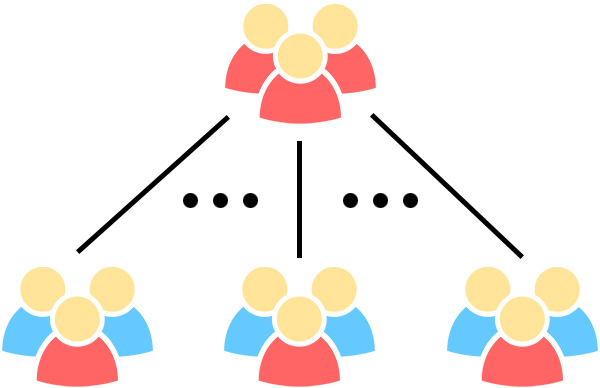
\includegraphics[height=.5\textheight]{pgraphics/scrum-of-scrums}

\end{frame}

\begin{frame}
\frametitle{Møder}

\begin{itemize}
\item Ugentlige statusmøder
\item Fælles sprint review
\item (Fælles) sprint planning
\end{itemize}

\end{frame}

\begin{frame}
\frametitle{Samarbejde}

\begin{itemize}
\item Fælles komponenter
\begin{itemize}
\item Database (OasisLib)
\item GUI (giraf-components)
\item (Mindre dele)
\end{itemize}
\item Værktøjer
\begin{itemize}
\item Redmine
\item Git
\item Jenkins
\end{itemize}
\item Specialister
\end{itemize}

\end{frame}

% % %
% CARS
% % %
\subsection{Cars}

\begin{frame}
\frametitle{Filosofi}

\begin{itemize}
\item Formål
\begin{itemize}
\item At hjælpe borgere med at udvikle deres stemme
\item Borgere der har problemer med at styre deres stemme
\item Borgere der har problemer med at vide hvilken stemme der passer til hvilken kontekst
\end{itemize}
\item Brug
\begin{itemize}
\item Pædagog sidder med borger og spiller spillet
\item Kan senere referere til spillet og barnet har nemmere ved at forholde sig til den stemme der skal ændres til
\end{itemize}
\end{itemize}

\end{frame}

\begin{frame}
\frametitle{Udvikling}

\begin{columns}

\begin{column}{.48\textwidth}
\begin{itemize}
\item Sprint 1
\begin{itemize}
\item Gamle krav
\item Styring via volume
\item Refaktorering (framework)
\end{itemize}
\item Sprint 2
\begin{itemize}
\item Begyndende implementering
\item Første interview
\item Nye krav
\end{itemize}
\end{itemize}
\end{column}

\begin{column}{.48\textwidth}
\begin{itemize}
\item Sprint 3
\begin{itemize}
\item Implementering af krav
\item Brug af database/GUI
\item Forbedring af styring
\end{itemize}
\item Sprint 4
\begin{itemize}
\item Vigtigste interview
\item Nye krav
\item Implementering af nye krav
\end{itemize}
\end{itemize}
\end{column}

\end{columns}

\end{frame}

\begin{frame}
\frametitle{Fremgangsmåde}

\begin{itemize}
\item Scrum
\item Morgenmøde
\item Scrumboard
\begin{itemize}
\item Stories
\item Tasks
\item Planning poker
\end{itemize}
\item Tasks ud fra krav
\end{itemize}

\end{frame}
\section{Kundekontakt / Krav}

\subsection{Interviews}

\begin{frame}
To interviews blev udført 

\begin{itemize}
\item 4. April, 2. sprint - to pædagoger fra Birken \\ Præcisering af gamle krav
\item 8. Maj, 4. sprint - talepædagog \\Feedback fra oprindelig kontaktperson på Cars 
\end{itemize}

\end{frame}

\begin{frame}{Metode}
\begin{itemize}
\item Semistruktureret interview 
\item Åbne spørgsmål - tillader de interviewede at komme med idéer og feedback
\end{itemize}
\end{frame}

\begin{frame}{Resultat}
\begin{itemize}
\item Præcisering af krav
\item Nye krav
\item Feedback på produktet
\end{itemize}
\end{frame}

\begin{frame}{Problemstillinger}
\begin{itemize}
\item Interview timing
\item Kunder skifter mening
\item Misforståelser
\end{itemize}
\end{frame}

\subsection{Kravstyring}


\begin{frame}{Fælleskrav}
\begin{itemize}
\item Krav fra det fællesprojekt
\item Uformelle 
\item Svære at holde styr på
\end{itemize}
\end{frame}

\begin{frame}{Opdatering af krav}
\begin{itemize}
\item Baseret på udførte interviews
\item Userstories, tasks
\item Dokumenteret i rapporten i tabeller
\end{itemize}
\end{frame}

\begin{frame}{Eksempel}
Fra original Cars rapport
\begin{itemize}
\item \textit{It must be possible for the user to change the difficulty of the game}
\end{itemize}

Efter første interview
\begin{itemize}
\item Speed is alterable. The speed level is represented as a digit between 0 and 10.
\item The placement and number of obstacles is alterable
%\item The placement of obstacles should be in such a way, that it is possible to adapt it to both citizen with tendency to speaking too loud as well as those speaking too low.
\item It should be possible, in settings, to switch\\ between avoiding objects and picking objects up.
\end{itemize}
\end{frame}

\section{Design}
\section{Videreudvikling}
\subsection{}
\begin{frame}
\frametitle{Demonstration}
\end{frame}
\begin{frame}
\frametitle{Videre udvilking}
Cars er \textit{''færdigt''}
\begin{itemize}
\item Alle krav opfyldt
\item Kun få tilbageværende problemer:
\begin{itemize}
\item Kalibrerings metode
\item Skalering af settings
\item Manglende test
\end{itemize}
\end{itemize}
\end{frame}

\end{document}